\section{Question 1}
Figure \ref{q1:frequencies} shows the dependencies obtained as suggested in the
lab handout.

\begin{figure}[htb]
  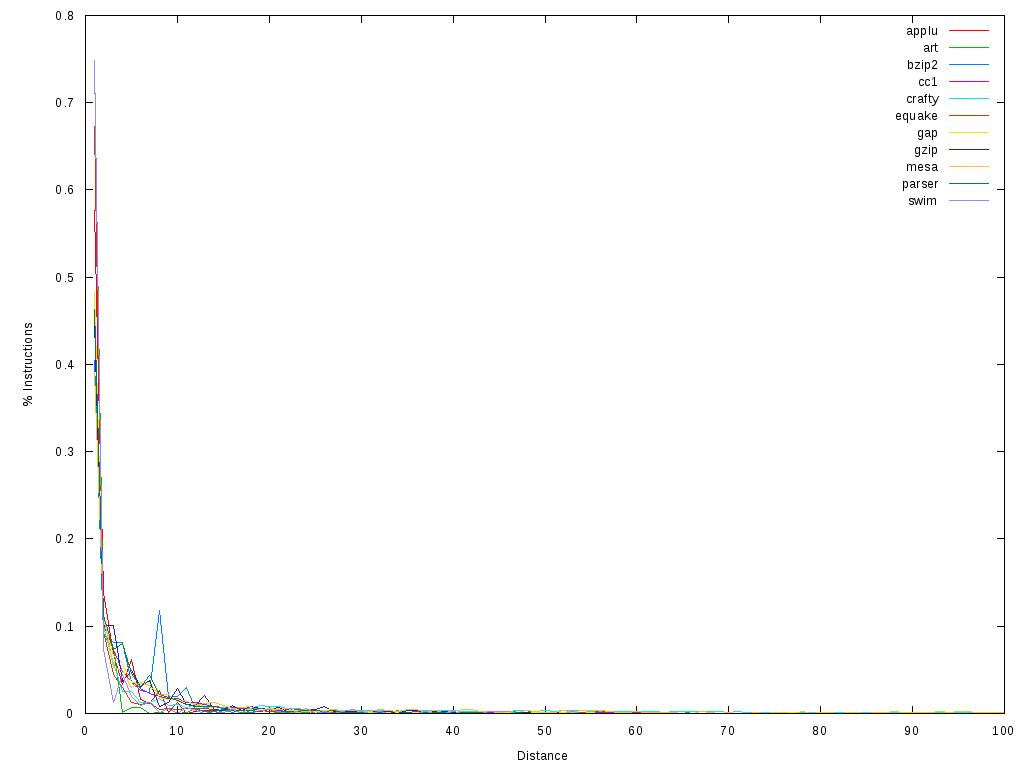
\includegraphics[width=6.8in]{6.823/lab1/figs/frequencies.png}
  \caption{Instruction dependency frequencies for the 11 benchmarks. }
  \label{q1:frequencies}.
\end{figure}

The graph is not too helpful, except to tell us that most instructions depend
on registers written in the past 4-5 instructions. Therefore, we use figure
\ref{q1:frequencies_zoom} to take a better look at the dependencies at most 5
instructions apart.

\begin{figure}[htb]
  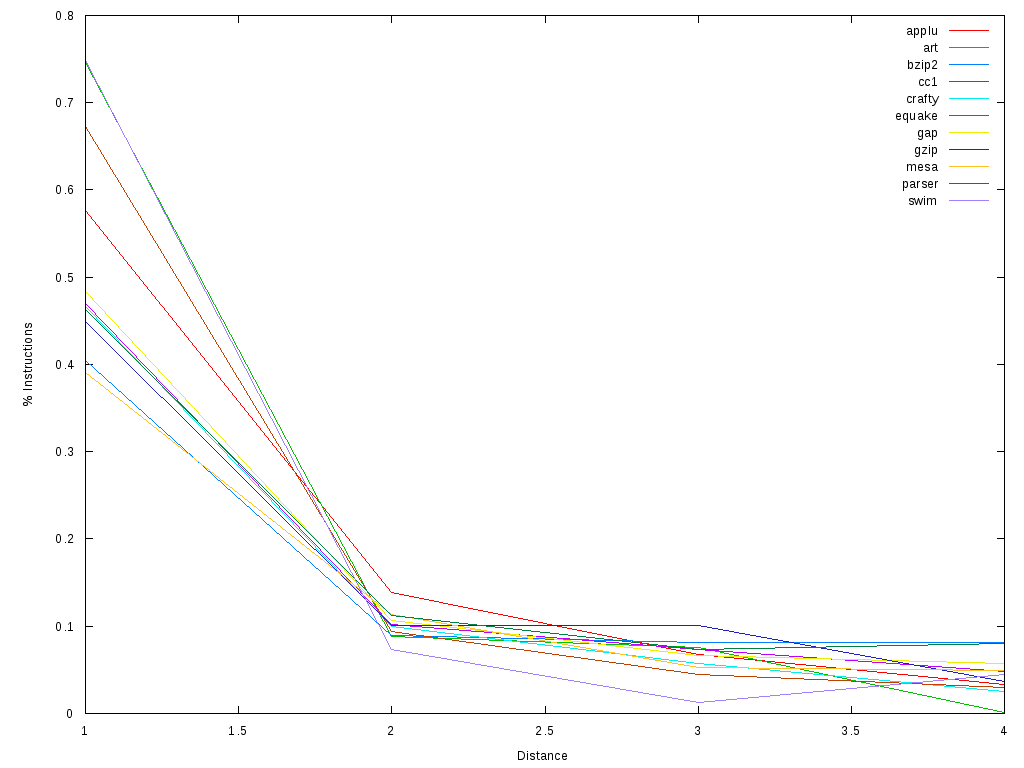
\includegraphics[width=6.8in]{6.823/lab1/figs/frequencies_zoom.png}
  \caption{Instruction dependency frequencies for the 11 benchmarks. }
  \label{q1:frequencies_zoom}.
\end{figure}

Given the dependency statistics, it seesms like architecture A would be
significantly faster than architecture B. In each benchmark, between 40\% -
80\% of the instructions depend on the previous instruction. In architecture B,
all instructions with dependencies on the previous instruction would have to be
stalled for 1 cycle, while the previous instruction writes its registers. This
means 40\%-80\% pipeline bubbles, which could be avoided by the forwarding
circuitry.

\section{Question 2}

Figure \ref{q2:reg_frequencies} shows the per-register breakdown for the
instruction dependency. For each register and instruction distance, we computed
the proportion of dependencies that are owed to that register. We averaged the
values for each benchmark. We only plotted registers which contributed a
dependency of at least 0.005\% on for at least one distance.

\begin{figure}[htb]
  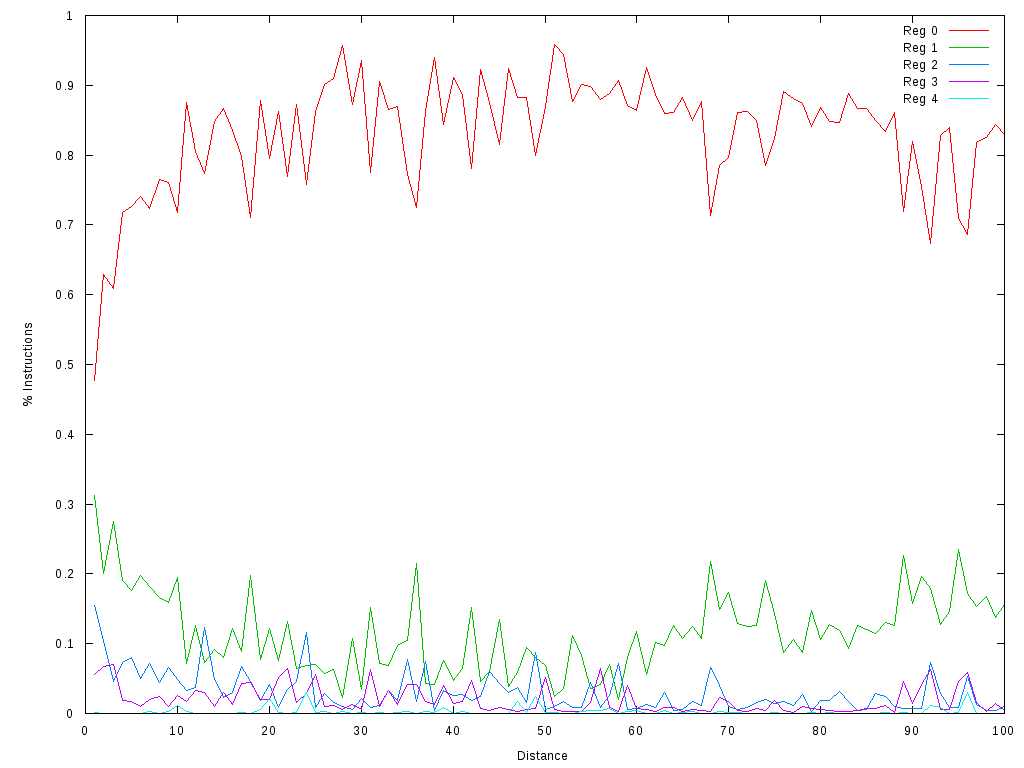
\includegraphics[width=6.8in]{6.823/lab1/figs/reg_frequencies.png}
  \caption{Instruction dependency frequencies broken down by register. }
  \label{q2:reg_frequencies}.
\end{figure}

The graph suggests that a few registers are responsible for most dependencies.
This is not very surprising, given the x86 architecture's predilection to use
the \texttt{eax} register as an accumulator, \texttt{esi} and \texttt{edi}
as pointers, and the presence of a condition flags register.

The best (but most difficult to implement) suggestion would be to give the
instruction set a makeover so it looks more like a RISC instruction set. It's
not cool to have 8 registers, and instructions with limitations on the registers
they can use. However, as Alpha found out, this strategy might not work
commercially.\footnote{One could argue that, even though the strategy failed in
the 1990s, we're living in a different landscape right now, where many servers
are running some flavor of UNIX/Linux. So, maybe the instruction set will be
redesigned one day.}

Assuming we're stuck with the ISA, it seems that (limited) forwarding is very
worth-while. The dependencies seem to taper off after 4 cycles, so it's
probably not worth forwarding for more than 4 cycles. This is important in
super-pipelined architectures, like the latest Pentiums and Core processors.

\section{Question 3}
The trade-off in the analysis is, in a nutshell, simpler code versus more
accurate results. Ironically, the best way to measure the trade-off is to
actually get the accurate results, and see the error. Table \ref{q3:mse} shows
the MSE (mean-square error) for the histograms for each test, as well as the
differences in the first 3 frequencies (for distance 1 up to distance 3).

\begin{figure}[htb]
\center
\begin{tabular}{lrrrr}
\hline
Test & MSE & Distance 1 & Distance 2 & Distance 3 \\
\hline
applu & 0.000\% & -0.000\% & +0.000\% & +0.000\% \\
\hline
art & 0.000\% & -0.000\% & +0.000\% & -0.000\% \\
\hline
bzip2 & 0.001\% & -0.000\% & +0.005\% & -0.000\% \\
\hline
cc1 & 0.001\% & -0.000\% & +0.006\% & -0.001\% \\
\hline
crafty & 0.002\% & +0.000\% & +0.014\% & -0.003\% \\
\hline
equake & 0.000\% & -0.000\% & +0.003\% & +0.001\% \\
\hline
gap & 0.001\% & -0.000\% & +0.003\% & -0.001\% \\
\hline
gzip & 0.001\% & -0.000\% & +0.006\% & -0.000\% \\
\hline
mesa & 0.002\% & +0.000\% & +0.013\% & +0.002\% \\
\hline
parser & 0.001\% & -0.000\% & +0.007\% & -0.001\% \\
\hline
swim & 0.000\% & -0.000\% & +0.000\% & +0.000\% \\
\hline
\end{tabular}

\caption{The MSE and differences in the first 3 frequencies between accurate
register accounting and approximating x86 8-bit and 16-bit partial registers
with the full-length register. }
\label{q3:mse}
\end{figure}

The tradeoff is not acceptable to me, since I'm a perfectionist, and I'd rather
write 100 lines of code (mostly obtained by copy-pasting 5 lines) to get
``perfect'' (exact) numbers.  However, from a technical perspective, the
trade-off is perfectly acceptable, because the inacurracy introduced (less than
1\%) should be significantly smaller than the inaccuracy of counting predicated
instructions (e.g. the \texttt{rep\_\textit{xx}} opcodes) once, instead of
accurately counting them.

\section{Question 4}

The graphs suggest that architecture B has less general-purpose registers than
architecture A. Assuming the compiler is decent (gcc3.4 fits the bill) and its
optimizations are turned on (which would be expected when running benchmarks),
I would expect that the compiler will try to minimize the dependencies between
adjacent instructions (it seems like a good idea, no matter what the pipeline
length is).

In fact, the huge proportion of distance-1 dependencies in architecture B (80\%)
makes me guess that the architecture either has very few registers, or some
opcodes force the use of a certain register as an accumulator (for example,
early Intel x86 processors forced one of the sources and the destination of {\tt
mul} and {\tt div} to be {\tt \%eax}, the ``accumulator'' register), or the
opcodes use the 2-register format ($r_t = r_d$).
